% !TeX program = xelatex
% Options for packages loaded elsewhere
\PassOptionsToPackage{unicode}{hyperref}
\PassOptionsToPackage{hyphens}{url}
\documentclass[
]{article}
\usepackage{xcolor}
\usepackage{amsmath,amssymb}
\setcounter{secnumdepth}{-\maxdimen} % remove section numbering
\usepackage{iftex}
\ifPDFTeX
  \usepackage[T1]{fontenc}
  \usepackage[utf8]{inputenc}
  \usepackage{textcomp} % provide euro and other symbols
\else % if luatex or xetex
  \usepackage{unicode-math} % this also loads fontspec
  \defaultfontfeatures{Scale=MatchLowercase}
  \defaultfontfeatures[\rmfamily]{Ligatures=TeX,Scale=1}
\fi
\usepackage{lmodern}
\ifPDFTeX\else
  % xetex/luatex font selection
\fi
% Use upquote if available, for straight quotes in verbatim environments
\IfFileExists{upquote.sty}{\usepackage{upquote}}{}
\IfFileExists{microtype.sty}{% use microtype if available
  \usepackage[]{microtype}
  \UseMicrotypeSet[protrusion]{basicmath} % disable protrusion for tt fonts
}{}
\makeatletter
\@ifundefined{KOMAClassName}{% if non-KOMA class
  \IfFileExists{parskip.sty}{%
    \usepackage{parskip}
  }{% else
    \setlength{\parindent}{0pt}
    \setlength{\parskip}{6pt plus 2pt minus 1pt}}
}{% if KOMA class
  \KOMAoptions{parskip=half}}
\makeatother
\usepackage{longtable,booktabs,array}
\newcounter{none} % for unnumbered tables
\usepackage{calc} % for calculating minipage widths
% Correct order of tables after \paragraph or \subparagraph
\usepackage{etoolbox}
\makeatletter
\patchcmd\longtable{\par}{\if@noskipsec\mbox{}\fi\par}{}{}
\makeatother
% Allow footnotes in longtable head/foot
\IfFileExists{footnotehyper.sty}{\usepackage{footnotehyper}}{\usepackage{footnote}}
\makesavenoteenv{longtable}
\usepackage{graphicx}
\makeatletter
\newsavebox\pandoc@box
\newcommand*\pandocbounded[1]{% scales image to fit in text height/width
  \sbox\pandoc@box{#1}%
  \Gscale@div\@tempa{\textheight}{\dimexpr\ht\pandoc@box+\dp\pandoc@box\relax}%
  \Gscale@div\@tempb{\linewidth}{\wd\pandoc@box}%
  \ifdim\@tempb\p@<\@tempa\p@\let\@tempa\@tempb\fi% select the smaller of both
  \ifdim\@tempa\p@<\p@\scalebox{\@tempa}{\usebox\pandoc@box}%
  \else\usebox{\pandoc@box}%
  \fi%
}
% Set default figure placement to htbp
\def\fps@figure{htbp}
\makeatother
\usepackage{svg}
\ifLuaTeX
  \usepackage{luacolor}
  \usepackage[soul]{lua-ul}
\else
  \usepackage{soul}
\fi
\setlength{\emergencystretch}{3em} % prevent overfull lines
\providecommand{\tightlist}{%
  \setlength{\itemsep}{0pt}\setlength{\parskip}{0pt}}
\usepackage{bookmark}
\IfFileExists{xurl.sty}{\usepackage{xurl}}{} % add URL line breaks if available
\urlstyle{same}
% fallback for those not using the hyperref driver hyperxmp:
\makeatletter
\@ifundefined{xmpquote}{\newcommand{\xmpquote}[1]{#1}}{}
\makeatother
\hypersetup{
  hidelinks,
  pdfcreator={LaTeX via pandoc}}

\author{}
\date{}

\begin{document}

\textbf{Non-extreme Rainfall and Tide Synchronization Driving Compound
Coastal Flooding in a Mega-delta}

Shuai Wang \textsuperscript{1,‡}, Yilong Niu \textsuperscript{2,‡}, Zhan
Tian \textsuperscript{3,*}, Laixiang Sun \textsuperscript{4,*}, Qinghua
Ye \textsuperscript{5}, Ralf Toumi \textsuperscript{6}, Guangtao Dong
\textsuperscript{7}, Md Musfike Meraz \textsuperscript{1}

\textsuperscript{1} Department of Geography and Spatial Sciences,
University of Delaware, DE, 19706, USA

\textsuperscript{2} yyyyyyyyyyy

\textsuperscript{3} School of Environmental Science and Engineering,
Southern University of Science and Technology, Shenzhen, 518055, China

\textsuperscript{4} Department of Geographical Sciences, University of
Maryland, College Park, MD, 20742, USA

\textsuperscript{5} Deltares, Delft, the Netherlands

\textsuperscript{6} Department of Physical, Imperial College London,
London, UK

\textsuperscript{7} Shanghai Climate Center, Shanghai Meteorological
Service, Shanghai, China

\textsuperscript{‡} Equal contribution

\textsuperscript{*} Corresponding authors:
\href{mailto:tianz@sustech.edu.cn}{\nolinkurl{tianz@sustech.edu.cn}},
\href{mailto:lsun123@umd.edu}{\nolinkurl{lsun123@umd.edu}}

\textbf{Abstract}

Catastrophic floods in coastal megacities are often attributed to rare
extremes in rainfall or storm surge, yet many occur under only moderate
forcing. We analyze the 1905 Shanghai flood to show how temporal
compounding of modest rainfall, storm tide and defense characteristics
generated extreme impacts in a mega-delta. Using historical pressure and
track data, we reconstruct the typhoon and force a two-dimensional
hydrodynamic model configured with river networks, bathymetry and
embankments. Long-term observations indicate that two antecedent
rainfall events (\textasciitilde2-year and \textasciitilde5-year return
periods) and a \textasciitilde10-year storm tide inundated 73\% of the
area, with depths \textgreater1 m across large districts. Factorial
experiments show that removing the second rainfall event or shifting the
storm tide from spring to neap conditions reduces inundation, and that
embankments redistribute rather than eliminate risk. The results reveal
a ``\emph{\textbf{return-period paradox}}'' and call for flood-risk
metrics and early-warning systems that explicitly account for temporal
compounding.

\textbf{Introduction}

Coastal megacities and deltas are widely recognized as hotspots of flood
risk under climate change, sea-level rise and rapid urbanization
\textsuperscript{1,2}. Their exposure is amplified by dense populations,
critical infrastructure and tightly interconnected economic systems,
while their low elevations and subsiding land surfaces constrain
drainage and compound the impacts of storm tides and heavy rainfall
\textsuperscript{3--5}. Conventional risk assessments and design
standards in these environments typically treat rainfall, storm surge
and tides as separate drivers, often characterized by univariate or
bivariate return periods \textsuperscript{6--8}. In practice, however,
many of the most damaging events have occurred not under record-breaking
extremes of any single driver, but under seemingly moderate
meteorological and hydrological forcing that interacted with antecedent
wetness, tidal phase and defense performance in time
\textsuperscript{9--12}.

The concept of compound flooding has emerged to describe events in which
multiple drivers co-occur or interact, such as simultaneous coastal
surge and fluvial discharge, or joint pluvial and fluvial extremes
\textsuperscript{13--16}. Existing studies have predominantly focused on
concurrence at or near the time of peak water level, quantifying joint
probabilities and dependence structures between drivers
\textsuperscript{9,17,18}. Much less attention has been given to what
might be termed ``temporally compounded'' events, where the critical
interaction arises from the sequencing of drivers over days rather than
from their exact coincidence in time. In such cases, antecedent rainfall
may saturate a catchment and fill storage, leaving the system primed
such that a later, only moderately high tide or surge triggers
widespread flooding \textsuperscript{19--21}. \emph{\textbf{These
temporally staggered compound events are difficult to diagnose from
statistical analyses alone}} because the key mechanism lies in evolving
system state rather than in the magnitude of any instantaneous forcing
\textsuperscript{9,19--21}.

Historical floods in pre-satellite, pre-radar eras offer underused
opportunities to understand temporal compounding in real-world settings.
Many such events are well documented in terms of impacts, water levels
and weather patterns, yet have seldom been revisited using modern
hydrodynamic models and long observational records. Mega-delta cities
are particularly valuable natural laboratories in this regard. Their
dense network of rivers, canals and embankments ensures that the
hydrodynamic response to combined rainfall, tide and surge is highly
nonlinear \textsuperscript{22,23}, while their long history of human
settlement has generated rich archival information on past disasters
\textsuperscript{24--26}. Reconstructing and numerically re-enacting
historical floods in these environments can therefore reveal which
combinations and sequences of drivers were most critical, and how
infrastructure and topography shaped the resulting inundation.

Shanghai, located in the Yangtze River Delta, is an archetypal coastal
megacity facing compound flood risks. In early September 1905, the city
suffered a catastrophic flood associated with a landfalling typhoon,
intense rainfall and elevated water levels along the Huangpu River and
adjacent coastal waters. Contemporary accounts describe widespread
inundation, disruption to transport and commerce, and severe damage to
housing and embankments, and identify the event as one of the deadliest
floods in the region, with tens of thousands of fatalities
\textsuperscript{27--29}. Yet available meteorological and oceanographic
records (shown later in the Results) indicate that neither the rainfall
nor the storm tide was exceptional when viewed in isolation; both fall
within ranges commonly used in present-day design standards. This
apparent discrepancy between moderate drivers and extreme impacts
illustrates a broader ``\emph{\textbf{return-period paradox}}'': urban
floods of great consequence arising from combinations of events that,
individually, would be considered frequent or manageable.

In this study, we use the 1905 Shanghai flood as a natural experiment to
quantify how temporal compounding of rainfall, tide and storm surge,
together with the configuration of flood defenses, produced catastrophic
inundation in a mega-delta city. We first reconstruct the responsible
typhoon using historical pressure and track data \textsuperscript{30}
and estimate the associated wind and pressure fields. These are used to
drive a two-dimensional hydrodynamic model configured with the early
twentieth-century coastline, river network, bathymetry and embankments
\textsuperscript{31}. Long-term observational records allow us to
estimate the return periods of the antecedent rainfall events and storm
tide that affected Shanghai in 1905, including century-scale tide-gauge
measurements in the region \textsuperscript{32}. We then design a suite
of numerical experiments that systematically modify the timing and
presence of antecedent rainfall, the tidal phase during the storm tide,
and the characteristics of coastal embankments, in order to attribute
flood extent and depth to specific processes and interactions.

Our objectives are threefold. First, we demonstrate that the 1905 flood
can be explained as the outcome of modest but temporally compounded
drivers in a highly constrained deltaic environment. Second, we identify
the relative contributions of antecedent rainfall, tide--surge
synchronization and defense configuration to the observed inundation
pattern, thereby clarifying the mechanisms of temporal preconditioning
and drainage blockage. Third, we discuss how these insights motivate the
development of flood-risk metrics, design standards and early-warning
systems that explicitly incorporate temporal compounding, moving beyond
traditional event-based approaches that focus on isolated extremes. By
reframing a historical catastrophe through the lens of compound
flooding, we highlight the need to consider not only how high the water
rises in coastal megacities, but also how the system is primed in the
days leading up to an event.

\textbf{Results}

\textbf{Non-extreme hydrometeorological drivers of the 1905 flood}

Today, tropical-cyclone (TC) tracks and intensity are routinely
monitored using satellite observations and global reanalysis, but such
information was unavailable in 1905. For the Shanghai event, we
therefore reconstructed the TC characteristics from historical
documentary sources and long instrumental records. The track of the 1905
typhoon was taken from the Atlas of the Tracks of 620 Typhoons
(1893--1918) \textsuperscript{ref.30}, which locates the storm center
passing to the southeast of Shanghai without direct landfall. To
estimate its intensity near Shanghai, we combined this track with
continuous surface pressure measurements from the Xujiahui Observatory,
which has operated continuously since the 1870s, and applied an
empirical statistical model that relates distance to the storm center
and local pressure deficit to central pressure and radius of maximum
wind (see Methods). The resulting parameters were used together with the
Holland wind profile implemented in the D-Flow FM hydrodynamic model to
generate a dynamically consistent wind and pressure field for the flood
simulations \textsuperscript{33,34}.

Historical records from Xujiahui indicate two pronounced rainfall events
preceding the main typhoon impact, on 21 August and 28 August 1905
(Figure 1). Because rain-gauge observations in 1905 were only available
at this single location, we assumed spatially uniform rainfall across
the model domain and prescribed the observed temporal rainfall series at
Xujiahui to all computational grid cells for the simulation period from
19 August to 3 September 1905. Using the long daily rainfall record at
Xujiahui (1874--2023), we then estimated the return periods of the two
antecedent rainfall events with a non-parametric method applied to
annual maxima of daily precipitation between 20 August and 3 September
of each year. The first event on 20--21 August produced 36.6 mm of
rainfall, corresponding to a return period of approximately 2 years
(31\textsuperscript{st} percentile of the seasonal annual maxima),
whereas the second event on 28 August produced 74.5 mm, corresponding to
a 5-year return period (62\textsuperscript{nd} percentile). Neither
rainfall episode would thus be classified as extreme in a conventional,
single-driver design framework.

The storm tide associated with the 1905 typhoon was reconstructed from
historical tide-gauge information at Wusongkou and a previous extreme
value analysis for the region \textsuperscript{35}, supported by long
tide-gauge records at Shanghai. The maximum total water level during the
storm reached about 5.4 m at Wusongkou (Figure 1), which corresponds to
a 10-year return period under early-twentieth-century conditions
\textsuperscript{32,35}. Taken in isolation, therefore, the three
principal hydrometeorological drivers -- the two antecedent rainfalls
and the storm tide -- all lie within the range typically considered
manageable for coastal infrastructure design. Yet contemporary accounts
describe the 1905 event as one of the most devastating floods in the
Shanghai region, with widespread inundation and substantial loss of life
\textsuperscript{27,29}. This apparent discrepancy foreshadows the
``return-period paradox'' central to our analysis: catastrophic flooding
emerging from the temporal compounding of individually non-extreme
drivers.

\textbf{Spatiotemporal evolution of inundation}

We first examine the simulated spatiotemporal evolution of inundation
during the 1905 event in the control experiment, in which both
antecedent rainfall events, the reconstructed storm tide, and the
historical embankment system are all included. Figure 1 summarizes the
time series of daily accumulated rainfall at Xujiahui and the simulated
astronomical tide and total water level at Wusongkou, while Figure 2
provides four representative snapshots of simulated water depth over the
model domain (see Supplementary Movie 1 for the full spatiotemporal
evolution of flooding).

Shortly after the first antecedent rainfall event on 21 August (Fig.
2a), simulated water depths remain mostly below 0.5 m across the
floodplain, with inundation confined to low-lying depressions and zones
adjacent to major river channels. Ponding is most apparent in the
northern and western parts of Shanghai, where limited drainage capacity
and flat topography favor local accumulation. These patterns indicate
that the first rainfall event alone was insufficient to generate severe
flooding, but it did initiate the filling of surface storage and the
wetting of soils, thereby modestly preconditioning the basin.

By contrast, the simulated inundation following the second antecedent
rainfall on 28 August (Fig. 2d) is more extensive and deeper. Flooded
areas expand both northwards and towards the historical urban core, and
local water depths reach 0.7--0.8 m in several districts. This reflects
the higher magnitude of the second rain event and, crucially, the fact
that it occurred over a system that had already been partially saturated
and hydraulically loaded by the first event. Reduced infiltration
capacity and diminished storage, together with limited artificial
drainage in 1905, lead to greater runoff coefficients and longer ponding
times. As a result, the modelled floodplain remains substantially
inundated even in the absence of additional rainfall during the days
preceding the typhoon.

The model state immediately before the arrival of the typhoon on 1
September (Fig. 2c) illustrates the degree of preconditioning. Despite
several dry hours, extensive shallow inundation persists over much of
the low-lying urban area and adjacent agricultural land. Embankment
systems along the Huangpu River and the coast are already hydraulically
stressed from inland water levels, and parts of the network of small
canals and creeks operate close to their conveyance capacity. In effect,
the catchment and the drainage network enter the typhoon stage with
limited residual buffering, so that even a moderate additional hydraulic
load can push the system beyond critical thresholds.

After the passage of the typhoon and the associated storm tide on 2
September (Fig. 2d), the compound nature of the event becomes fully
apparent. The simulated maximum inundation extent covers approximately
73\% of the modelled Shanghai area, and water depths exceed 1 m across
large contiguous regions, particularly in low-lying eastern districts
near the 1905 coastline. The interaction between inland flood-waters and
elevated coastal water levels prevents effective drainage, causing
backwater effects along the Huangpu and its tributaries and promoting
lateral overflow onto the floodplain. The overall pattern and depth of
simulated inundation are consistent with contemporary descriptions of
widespread, knee- to waist-deep flooding in the city and surrounding
counties \textsuperscript{27,29,36}, lending confidence to the
reconstructed event (see also the model validation in Methods).
Together, these simulations demonstrate that the catastrophic impact of
the 1905 flood cannot be attributed to any single extreme driver, but
rather to the way in which modest antecedent rainfall, limited drainage,
and the timing of the storm tide combined in a nonlinear way over
several days.

\textbf{Attribution of flood severity to antecedent rainfall, tide phase
and embankments}

To quantify the relative contributions of individual drivers to the
observed compound flooding, we conducted a set of sensitivity
experiments in which we systematically removed or modified key
hydrological and infrastructural factors while keeping all other
conditions unchanged. Specifically, we considered four perturbed
scenarios relative to the control run: (i) removal of the first
antecedent rainfall event (No-Rain-1), (ii) removal of the second
antecedent rainfall event (No-Rain-2), (iii) replacement of the spring
high tide with a neap high tide during the storm tide (Neap-Tide), and
(iv) substitution of the historical stone embankment system with lower
earthen embankments along the southern coast, similar to those
documented in the eastern coastal zone at the time (Earthen-Embankment).
The differences between each perturbed simulation and the control
isolate the role of individual factors in setting flood depth, extent
and spatial pattern.

The spatial patterns of depth differences are shown in Figure 3. In the
No-Rain-1 experiment (Fig. 3a), water depth reductions relative to the
control are confined to a limited fraction of the domain, mainly in
upstream catchment areas and local depressions where the first rainfall
contributed most to pre-event storage. The total flooded area remains
unchanged at 73\%, and only 11\% of the region experiences a decrease in
water depth. The 95th-percentile reduction in depth is modest, at 0.08 m
(Table 1). These metrics confirm that, while the first antecedent
rainfall event initiated preconditioning, its contribution to the
ultimate severity of the compound flood was relatively small.

In contrast, removing the second antecedent rainfall event produces far
more substantial changes. The No-Rain-2 simulation (Fig. 3b) exhibits
widespread reductions in flood depth across 63\% of the model domain,
with the largest decreases occurring in the central and northern urban
areas and along key drainage pathways. The 95th-percentile depth
reduction reaches 0.11 m, and shallow flooding retreats from several
districts that were inundated in the control run (Table 1). Despite
these reductions, the total flooded area remains large because the storm
tide and residual water from the first rainfall still generate extensive
inundation in low-lying zones. Nevertheless, the comparison between
No-Rain-1 and No-Rain-2 clearly indicates that the second rainfall
episode was the dominant hydrological preconditioner, consistent with
its higher magnitude and shorter temporal separation from the typhoon.
This asymmetric sensitivity also exemplifies the importance of event
sequencing: it is not merely the cumulative rainfall, but the timing of
individual pulses relative to the system's evolving state, that controls
compound flood potential \textsuperscript{9,19--21}.

The influence of tide phase is even more striking. In the Neap-Tide
experiment (Fig. 3c), replacing the spring high tide with a neap high
tide during the storm leads to a pronounced mitigation of flooding. The
proportion of the domain experiencing inundation drops from 73\% in the
control to 50\%, and 73\% of the area shows reduced water depths, with a
95th-percentile reduction of 1.02 m (Table 1). Depth decreases greater
than 0.3 m occur widely across the low-lying northeast and the inland
urban core, particularly near major river mouths and drainage basins.
Physically, this behavior reflects the role of high spring tides in
limiting the capacity of rivers and drainage channels to discharge
runoff to the sea. When the storm tide coincides with a spring high
tide, elevated coastal water levels generate strong backwater effects,
raising water surfaces far inland and amplifying the contribution of
antecedent rainfall to flooding. Under neap-tide conditions, by
contrast, the drainage system retains more freeboard and hydraulic
gradient, allowing part of the inland floodwater to be evacuated even as
the storm passes. These results demonstrate that tide--surge
synchronization is a first-order control on compound flood severity in
the Shanghai mega-delta, in line with recent studies of compound
surge--river events in other coastal systems \textsuperscript{9,17,18}.

The Earthen-Embankment experiment (Fig. 3d) illuminates the complex role
of structural defenses in shaping flood risk. Replacing the historical
stone embankments with lower, less resistant earthen structures
substantially increases flood exposure along the southern coastal zone.
In this scenario, the total flooded area expands to 78\% of the domain,
with 12\% of the area experiencing increased water depths; the
95th-percentile depth increase reaches 0.61 m (Table 1). Large parts of
the southern coastline that remained unflooded in the control run become
inundated, with depth increases exceeding 0.4 m. At the same time,
around 26\% of the area exhibits decreased depths, particularly in some
inland zones where the earlier presence of strong embankments
constrained overbank flow and promoted deeper ponding. When these
barriers are weakened, floodwaters can spill more freely across the
landscape, redistributing volumes from inland storage towards the coast.
This pattern underlines that embankments may reduce risk locally while
redistributing it spatially, a phenomenon also observed in modern levee
systems worldwide \textsuperscript{37,38}.

In summary, the sensitivity experiments highlight the strongly nonlinear
and temporally compounded nature of the 1905 Shanghai flood. Moderate
but sequential rainfall events primed the catchment and drainage
network; spring-tide conditions during the storm strongly inhibited
runoff evacuation and magnified inland water levels; and coastal
embankments provided local protection while reshaping the spatial
footprint of inundation. The catastrophe resulted not from any
individually exceptional driver, but from their combined timing and
interaction in a constrained mega-delta environment. These findings
challenge conventional approaches that assess coastal flood risk largely
through univariate or bivariate return periods of rainfall or storm tide
\textsuperscript{6--8,17,18,39--41} and instead point to the need for
state-dependent, temporally explicit metrics that capture how preceding
conditions and tide--surge synchronization can turn otherwise modest
hydrometeorological events into devastating floods.

\textbf{Discussion}

This study revisits the catastrophic 1905 flood in Shanghai as a natural
experiment in compound coastal flooding in a mega-delta city. By
reconstructing the responsible typhoon from historical track and
pressure data and driving a two-dimensional hydrodynamic model
configured for early twentieth-century conditions, we show that the
disaster did not arise from record-breaking rainfall or storm tide.
Instead, it resulted from the temporal compounding of two modest
antecedent rainfall events, a 10-year storm tide and the configuration
of embankments and drainage in a low-lying, hydraulically constrained
deltaic environment. The two rainfall events correspond to return
periods of only about 2 and 5 years, respectively, and the storm tide to
about 10 years, yet their combined effect produced simulated inundation
over \textasciitilde73\% of the Shanghai area, with water depths
exceeding 1 m across extensive districts, consistent with contemporary
documentary evidence of widespread, deep flooding and major loss of
life.

Our sensitivity experiments clarify the mechanisms by which such
non-extreme drivers generated extreme impacts. Removing the first
antecedent rainfall event has little influence on flood extent and
depth, whereas removing the second event reduces water levels across
much of the domain, highlighting the asymmetric role of event sequencing
and catchment preconditioning. The second and larger rainfall pulse
occurred when the system had already lost part of its storage capacity
and exhibited reduced infiltration, so that more of the precipitation
contributed directly to runoff. The neap-tide experiment reveals that
shifting the storm tide from spring to neap conditions substantially
mitigates flooding, reducing inundated area from 73\% to 50\% and
lowering the 95th-percentile water depth by \textasciitilde1 m. This
strongly points to tide--surge synchronization as a first-order control
on compound flood severity, consistent with recent work that emphasizes
the importance of timing and dependence between storm surge and fluvial
discharge in coastal systems. Together, these results illustrate a
``return-period paradox'': flood disasters in mega-deltas can emerge
from relatively frequent events when antecedent wetness, tidal phase and
surge coincide in time.

The embankment sensitivity experiment further shows that structural
defenses modify not only the magnitude but also the spatial distribution
of risk. In the control case, stone embankments reduce overtopping and
direct coastal inundation along the southern shore, but also constrain
flow paths and promote deeper ponding in some inland areas. When we
replace these structures with lower earthen embankments, flooding
increases markedly along the southern coastline and the overall
inundated area rises to 78\%, but water depths decrease in some inland
districts as floodwaters are redistributed more evenly across the
landscape. This pattern echoes broader evidence that levees and
embankments can reduce risk for some communities while transferring it
to others, underscoring the need to consider integrated system behavior
and not only local levels of protection when planning structural
measures in deltas.

Our findings have several implications for compound flood risk
assessment and management in coastal megacities. First, they demonstrate
that traditional design approaches based on univariate or bivariate
return periods of rainfall and storm tide are insufficient in
environments where system state and tidal phase strongly modulate the
response \textsuperscript{9,17,18,39,41--43}. Approaches that specify,
for example, a ``1-in-100-year'' storm tide or rainfall event do not
necessarily capture the probability of a particular multi-day sequence
of rainfall, basin wetness and tide--surge conditions that can trigger
catastrophic flooding. Instead, risk metrics need to become explicitly
state-dependent, incorporating the evolving storage and saturation
conditions of catchments and drainage networks as well as the timing of
coastal water-level extremes. This argues for compound event frameworks
that consider sequences (e.g., ``wet--wet--storm tide'' trajectories)
and their joint probabilities, rather than focusing solely on
instantaneous extremes.

Second, the results highlight priorities for early warning systems and
operational flood management. In many coastal cities, warnings are still
issued primarily based on forecasts of peak tide, surge or rainfall
intensity. Our analysis suggests that, for mega-deltas, effective
warning and preparedness should also monitor and forecast antecedent
basin wetness, the residual storage capacity of canals and floodplains,
and the expected alignment of storm surge with spring or neap tides.
Integrating hydrological and hydrodynamic state variables into
forecasting systems, alongside meteorological drivers, would help
identify periods when even moderate incoming storms may pose
disproportionate risk because the system is already near critical
thresholds \textsuperscript{9,19--21}. In practice, this could translate
into multi-stage warnings that escalate not only with predicted storm
intensity but also with indicators of preconditioning, such as soil
moisture indices, reservoir levels, or canal stage.

Third, historical reconstructions such as the one presented here can
play a unique role in stress-testing mega-delta cities. Instrumental
records of surge, tide and rainfall are typically only a few decades
long, which limits the direct statistical characterization of rare
compound sequences. Historical events, however, often predate modern
observation networks yet are documented qualitatively and, increasingly,
through early tide gauges, rain gauges and meteorological archives. By
combining these sources with physically based models, it becomes
possible to explore how particular sequences and infrastructure
configurations have produced extreme flooding in the past, and to test
the sensitivity of outcomes to hypothetical changes in embankments,
drainage or land use \textsuperscript{27--29,37,38}. Our Shanghai case
study illustrates that such reconstructions can provide detailed process
understanding and quantitative insight into the contribution of temporal
compounding, which is difficult to obtain from statistical analysis
alone.

The implications of this work extend beyond historical Shanghai. Many of
the world's major mega-deltas and coastal conurbations share key
characteristics with early-twentieth-century Shanghai: low elevations
close to mean sea level, extensive networks of natural and artificial
channels, reliance on embankments and seawalls, rapid land-use change
and subsidence, and exposure to tropical or extratropical cyclones
\textsuperscript{9,17,18,37--39,41--43}. As sea levels continue to rise
and extreme precipitation intensifies under climate change, the
likelihood that modest storms interact with high tides, elevated mean
sea levels and saturated catchments to produce devastating floods is
expected to increase. Our results suggest that adaptation strategies
focusing solely on raising defenses to meet higher design water levels
may underperform if they do not account for how system preconditioning
and tide--surge synchronization change under future climates and
socio-technical configurations. Integrating temporal compounding into
adaptation planning, for example through scenario-based simulations that
explore a range of multi-day sequences under different defense designs,
could help identify robust strategies that perform well across diverse
compound-event pathways.

Several limitations of this study should be acknowledged. First, the
reconstruction of the 1905 typhoon is subject to uncertainties in
historical track positions and surface pressure measurements, which
propagate into the estimated wind and pressure fields used to drive the
hydrodynamic model. Second, rainfall observations were available only at
the Xujiahui station, requiring us to assume spatially uniform
precipitation across the domain. This simplification may misrepresent
local runoff generation patterns, although the large-scale
preconditioning signal is likely captured adequately given the modest
size of the catchment relative to typical storm structures. Third, the
historical topography, river network and embankment elevations are
reconstructed from cartographic and documentary sources and thus carry
uncertainties, particularly in small-scale features that can influence
local flow paths. Finally, our model is depth-averaged and does not
include morphological change or sediment dynamics, which may affect
channel conveyance and defense performance over longer timescales.
Despite these limitations, the key qualitative findings, such as the
dominance of temporal compounding over individual driver extremeness,
the critical role of tide--surge synchronization, and the
risk-redistribution effects of embankments, are robust across a wide
range of plausible parameter choices and reconstruction assumptions.
They point to the need for compound flood risk assessments that move
beyond traditional event-based design and towards a trajectory-based
perspective in which the timing and sequence of meteorological,
hydrological and coastal processes are central. For coastal megacities
and mega-deltas, considering how the system is primed in the days
preceding a storm may be as important as estimating the storm's peak
intensity itself.

\st{\hfill\break
}

\textbf{Methods}

\subsection{\texorpdfstring{\textbf{Historical event and data
sources}}{Historical event and data sources}}\label{historical-event-and-data-sources}

We treat the September 1905 Shanghai flood as a natural experiment in
compound coastal flooding and compile a set of qualitative and
quantitative data to characterize both the event and its physical
environment. Contemporary documentary records, including the
Encyclopedia of Meteorological Disasters in China and local newspaper
reports, provide information on the date, duration and impacts of the
flood, as well as descriptive accounts of inundation depth and spatial
extent. These sources identify the event as one of the most damaging
floods in the Shanghai region in the late Qing period, with widespread
disruption to transport and commerce and substantial loss of life.

Cartographic and infrastructural information is taken primarily from the
Comprehensive Map of Songjiang Prefecture (1909) and related archival
materials, which describe the coastline, the Huangpu River and its
tributaries, smaller canals, and the locations of stone and earthen
embankments around Shanghai at the beginning of the twentieth century,
which is still visible/accessible in today's site visit. These maps form
the basis for reconstructing the historical drainage network and defense
system used in the hydrodynamic inundation model.

Meteorological observations are drawn from the long daily records at the
Xujiahui Observatory (now the Shanghai Meteorological Bureau), which has
operated since the 1870s. We use daily precipitation and surface
pressure data from 1874--2023 to characterize the rainfall and pressure
conditions associated with the 1905 event and to estimate return periods
of the antecedent rainfall episodes. Typhoon track information is
obtained from the Atlas of the Tracks of 620 Typhoons (1893--1918),
which provides six-hourly positions of the storm center for the 1905
tropical cyclone affecting Shanghai \textsuperscript{30}.

Ocean water-level data and long tide-gauge records from Wusongkou and
Shanghai are used to reconstruct the storm tide during the event and to
estimate its return period under early twentieth-century sea level.
These records also support the vertical datum corrections applied to
historical topography and embankment elevations.

Together, these archival, cartographic and instrumental datasets provide
the observational foundation for reconstructing the meteorological and
hydrodynamic drivers of the 1905 flood. In the following subsections we
describe how we use these data to (i) reconstruct storm wind and
pressure fields, (ii) estimate the rarity of the rainfall and storm
tide, and (iii) build a historical hydrodynamic model of the Shanghai
mega-delta.

\subsection{\texorpdfstring{\textbf{Reconstruction of typhoon wind and
pressure
fields}}{Reconstruction of typhoon wind and pressure fields}}\label{reconstruction-of-typhoon-wind-and-pressure-fields}

Building on the track and pressure data described above, we reconstruct
the three-dimensional wind and pressure fields of the 1905 typhoon to
force the hydrodynamic simulations. The storm track from the Atlas of
the Tracks of 620 Typhoons (1893--1918) provides six-hourly storm center
positions. For each time-step we compute the great-circle distance
\emph{R\textsubscript{sh}} between the storm center and Shanghai
(Xujiahui) and combine this with the observed surface pressure
\emph{P\textsubscript{sh}} at Xujiahui to infer the storm's central
pressure \emph{P\textsubscript{min}} and radius of maximum wind
\emph{R\textsubscript{max}}.

We adopt the analytical λ-model for tropical-cyclone wind profiles
\textsuperscript{44,45}, which relates central pressure, environmental
pressure \emph{P\textsubscript{env}}, \emph{R\textsubscript{max}}, and
radial distance \emph{R\textsubscript{sh}} to the local pressure and
wind fields. Using the observed \emph{P\textsubscript{sh}} and the
best-track distance \emph{R\textsubscript{sh}}, we invert the λ-model to
obtain time series of \emph{P\textsubscript{min}} and
\emph{R\textsubscript{max}} for the 1905 event. The resulting
\emph{P\textsubscript{min}} values are then converted to maximum
sustained winds using established wind--pressure relationships for
western North Pacific tropical cyclones \textsuperscript{33}.

To obtain spatially distributed wind and pressure fields, we apply the
Holland profile \textsuperscript{46,47}, parameterized by the inferred
\emph{P\textsubscript{min}}, \emph{P\textsubscript{env}},
\emph{R\textsubscript{max}} and scaling coefficient B, on a polar grid
centered on the storm track and interpolate these fields onto the
unstructured computational mesh of the D-Flow FM model. This yields
time-varying wind stress and atmospheric pressure forcing for the
hydrodynamic simulations. More details on the reconstruction of 1905
typhoon can be found in Supplementary Text 1.

This reconstruction links sparse historical observations to a physically
consistent forcing dataset for the flood model. We next describe how we
characterize the rainfall events and storm tide associated with the
compound flooding.

\subsection{\texorpdfstring{\textbf{Rainfall events and return-period
estimation}}{Rainfall events and return-period estimation}}\label{rainfall-events-and-return-period-estimation}

To quantify the rarity of the rainfall drivers of the 1905 flood, we use
the long daily precipitation record at Xujiahui for the period
1874--2023. We first identify the two main antecedent rainfall episodes
preceding the typhoon, occurring on 21 August and 28 August 1905
respectively, and compute their daily totals. Because we are interested
in events occurring in the same part of the seasonal cycle, we extract,
for each year, the maximum daily rainfall during the window 20 August--3
September.

We then estimate empirical return periods for the 1905 daily totals
using a non-parametric plotting-position approach applied to this
seasonal-window series. The smaller 21 August event (36.6 mm day⁻¹)
corresponds to approximately a 2-year return period, while the larger 28
August event (74.5 mm day⁻¹) corresponds to around 5 years. These
estimates confirm that neither antecedent rainfall episode is extreme in
a univariate sense.

Rainfall observations in 1905 are only available at Xujiahui; spatial
rainfall patterns during individual storms are therefore unknown. We
approximate spatial rainfall in the hydrodynamic simulations by applying
the observed Xujiahui time series uniformly across the model domain for
the period 19 August--3 September 1905. While this simplification
neglects sub-domain variability, it captures the key temporal structure
of the antecedent wetting and the main rainfall pulses, which is most
relevant to basin preconditioning and temporal compounding.

Having characterized the rainfall sequence, we next describe how we
reconstruct the storm tide and water-level return periods for the
coastal boundary conditions.

\subsection{\texorpdfstring{\textbf{Storm-tide reconstruction and
vertical datum
corrections}}{Storm-tide reconstruction and vertical datum corrections}}\label{storm-tide-reconstruction-and-vertical-datum-corrections}

The total water level at the coastal boundary during the 1905 event is
reconstructed from historical tide-gauge information at Wusongkou and an
extreme-value analysis for Shanghai and neighboring stations. Historical
records and prior analysis indicate that the maximum storm tide reached
approximately 18 ft 6 in (≈ 5.6 m) at Wusongkou during the event. To
relate this to our model and to estimate its return period, we make two
key adjustments.

First, we correct historical water-level and topographic data for
vertical datum differences between early twentieth-century surveys and
modern chart datums, based on documented offsets of about 1.659 m in the
Shanghai region. Second, we account for mean sea-level rise between the
early 1920s and the present, estimated at approximately 0.357 m using
long tide-gauge records. The combined 2.016 m adjustment is applied to
the historical coastline, riverbanks and embankment elevations to ensure
consistency between reconstructed 1905 levels and the model's vertical
reference.

We superimpose an astronomical tide and a storm-surge component to
generate the total water-level boundary condition at Wusongkou. For the
control simulation, the storm tide coincides with a spring high tide,
consistent with documentary evidence and previous analyses, while in the
Neap-Tide sensitivity experiment we replace the spring tide component
with a representative neap high tide while preserving the surge shape
and timing.

These reconstructions yield boundary water-level conditions whose
magnitude corresponds to approximately a 10-year return period under
early twentieth-century sea level. We now turn to the representation of
the historical land surface, drainage network and embankment system on
which these drivers acted.

\subsection{\texorpdfstring{\textbf{Historical topography, drainage
network and
embankments}}{Historical topography, drainage network and embankments}}\label{historical-topography-drainage-network-and-embankments}

The historical physical setting of Shanghai is represented using a
combination of topographic data, historical mapping, and archival
descriptions of embankments and channels. We begin with a regional
digital elevation model (DEM) covering the lower Huangpu River and
adjacent floodplains, which is adjusted to align with the 1909
Comprehensive Map of Songjiang Prefecture and other contemporaneous
maps. Elevations are corrected for vertical datum differences and mean
sea-level rise as described above.

The historical drainage network---including the Huangpu River, its
tributaries, canals and smaller creeks---is digitized from the 1909 map
and integrated into the unstructured model mesh. Historical embankments
are classified as stone or earthen based on textual descriptions and map
symbology, with crest locations and approximate heights assigned
accordingly. Stone embankments along the southern coast of Shanghai are
represented as higher, more resistant features, whereas earthen
embankments in the eastern coastal zone are assigned lower crest
elevations and different roughness characteristics.

Where available, historical information on land use and urbanization is
used to distinguish between built-up and rural areas in assigning
surface roughness and infiltration parameters, though the representation
remains necessarily simplified given data limitations in 1905.

This historical configuration provides the spatial template for the
hydrodynamic simulations, representing the system state against which
the temporally compounded rainfall and storm tide sequence plays out. We
next describe the hydrodynamic inundation model used to simulate flood
extents and depths.

\subsection{\texorpdfstring{\textbf{Hydrodynamic model
set-up}}{Hydrodynamic model set-up}}\label{hydrodynamic-model-set-up}

We use the two-dimensional depth-averaged D-Flow FM model to simulate
the inundation of the lower Huangpu River and surrounding area during
the 1905 event. The model domain encompasses the coastal zone near
Wusongkou, the lower reaches of the Huangpu River, and the historical
urban and peri-urban areas of Shanghai, extending sufficiently inland to
capture overbank inundation.

The unstructured computational mesh is refined along main channels and
embankments to better resolve flow paths and overtopping, with coarser
resolution in offshore areas. Open-boundary conditions include the
time-varying water level at Wusongkou, reconstructed as described above,
and prescribed or free-outflow conditions at upstream river boundaries,
depending on data availability. Wind stress and atmospheric pressure
fields derived from the typhoon reconstruction are applied uniformly
over the model domain at each time step.

Rainfall is applied as a uniform areal source term using the Xujiahui
precipitation time series for 19 August--3 September 1905. Bottom
friction is represented using spatially varying Manning or Chézy
roughness coefficients, with higher roughness assigned to urban and
vegetated floodplains and lower values in main channels. Embankments are
incorporated as elevated linear features following their historical
alignments, with crest elevations and roughness parameters
differentiating stone and earthen structures.

Simulations are run from 00:00 on 19 August to 21:00 on 2 September
1905, encompassing the two antecedent rainfall events and the main
typhoon impact. Model outputs include hourly maps of water depth and
water level at key points, which are used to derive maximum inundation
extents and depths for each experiment.

With the hydrodynamic model in place, we design a set of experiments to
isolate the role of temporal compounding and infrastructure
configuration in shaping the 1905 flood.

\subsection{\texorpdfstring{\textbf{Experimental design for temporal
compounding}}{Experimental design for temporal compounding}}\label{experimental-design-for-temporal-compounding}

To attribute the severity and spatial pattern of the 1905 flood to
individual drivers and their sequencing, we employ a factorial
experimental design. The control experiment includes both antecedent
rainfall events (21 August and 28 August), the reconstructed spring-tide
storm tide, and the historical stone and earthen embankment system,
representing our best estimate of the actual 1905 conditions.

We then define four sensitivity experiments, each modifying a single key
factor while holding all others constant:

\begin{quote}
1. No-Rain-1: the first antecedent rainfall event (21 August) is removed
from the forcing, while the second rainfall event, storm tide and
embankment configuration remain unchanged.

2. No-Rain-2: the second antecedent rainfall event (28 August) is
removed, while retaining the first rainfall event, storm tide and
embankments.

3. Neap-Tide: the spring high tide coinciding with the storm tide in the
control simulation is replaced by a representative neap high tide,
preserving the surge's timing and shape but increasing coastal drainage
capacity.

4. Earthen-Embankment: stone embankments along the southern coast are
replaced by earthen embankments with lower crest elevations and
different roughness coefficients, consistent with archival descriptions
for the eastern coastal zone.
\end{quote}

For each experiment, we compute maximum water depth over the simulation
period and derive scalar metrics of flood severity: total flooded area,
percentage of the domain experiencing depth increases or decreases
relative to the control, and the 95th-percentile depth and depth
differences. Spatial maps of depth differences (experiment minus
control) are used to diagnose where and how changes in each driver
modify inundation.

By comparing these experiments to the control, we isolate the
contributions of antecedent rainfall, tide phase and embankment
configuration to the compound flood outcome. In the final subsection we
describe how we validate the model and assess key sources of
uncertainty.

\subsection{\texorpdfstring{\textbf{Model validation and uncertainty
analysis}}{Model validation and uncertainty analysis}}\label{model-validation-and-uncertainty-analysis}

We validate the hydrodynamic model against both quantitative water-level
information and qualitative descriptions of inundation during the 1905
event. At Wusongkou, the model reproduces the timing and magnitude of
the reported storm tide peak, with simulated maximum water level of
\textasciitilde5.4 m compared to the historical estimate of 18 ft 6 in
(≈ 5.6 m), after accounting for datum and sea-level corrections. Time
series of water level at other locations along the Huangpu River are
qualitatively consistent with reported patterns of elevated river
stages.

Spatially, the simulated maximum inundation extent in the control
experiment covers \textasciitilde73\% of the historical Shanghai area,
and water depths exceed 1 m across large districts in the eastern and
central parts of the city. These patterns align with documentary
accounts of widespread, knee- to waist-deep flooding in the urban core
and surrounding counties, as well as with reports that embankments along
the southern coast largely prevented direct coastal overtopping in that
sector.

Uncertainties remain in several aspects of the reconstruction. The
typhoon intensity and wind field are subject to uncertainties in
historical track positions, the λ-model parameterization, and the
wind--pressure relationships used. Rainfall is assumed spatially uniform
due to lack of additional gauges, which may misrepresent local runoff
generation. The historical DEM, river network and embankment heights are
reconstructed from maps and textual descriptions and may not capture
fine-scale elevation and structural details. Moreover, the
depth-averaged hydrodynamic model neglects vertical stratification and
sediment dynamics, which could affect channel conveyance on longer
timescales.

To partially mitigate these uncertainties, we focus interpretation on
relative differences between the control and sensitivity experiments,
which are less sensitive to absolute biases in forcing and topography
because all simulations share the same underlying reconstruction. Across
plausible variations in reconstruction parameters tested in
supplementary experiments, the qualitative conclusions regarding the
roles of antecedent rainfall, tide--surge synchronization and embankment
configuration remain robust.

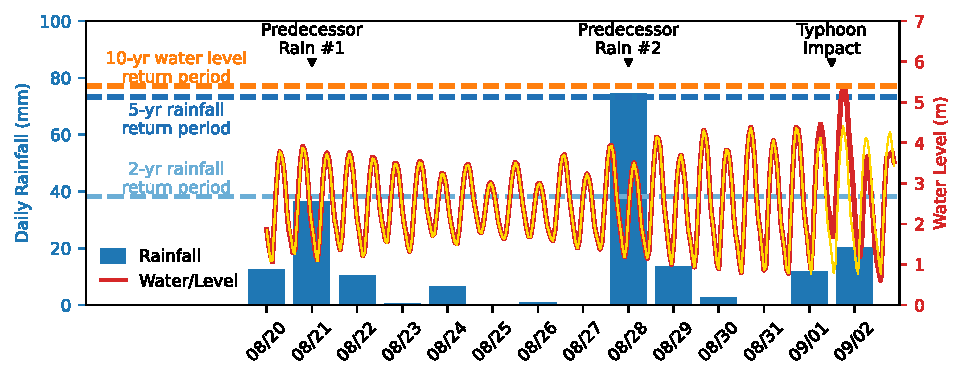
\includegraphics[width=6.41667in,height=2.52778in]{media_main/media/image2.pdf}

Figure 1. Time series of daily accumulated rainfall (mm) observed in
Xujiahui (blue bar), and astronomical tide (yellow solid line) and total
simulated water depth (red solid line) at Wusongkou gauge station. The
blue dashed lines show 5-yr and 2-yr return periods of daily accumulated
rainfall amount based on the non-parametric estimation with annual
maximum daily rainfall observations in Xujiahui from August
20\textsuperscript{th} to September 3\textsuperscript{rd} for 1874-2023.
The orange dashed line shows the 10-yr return period of water level at
Wusongkou station based on the estimation from a period study
\textsuperscript{35}.

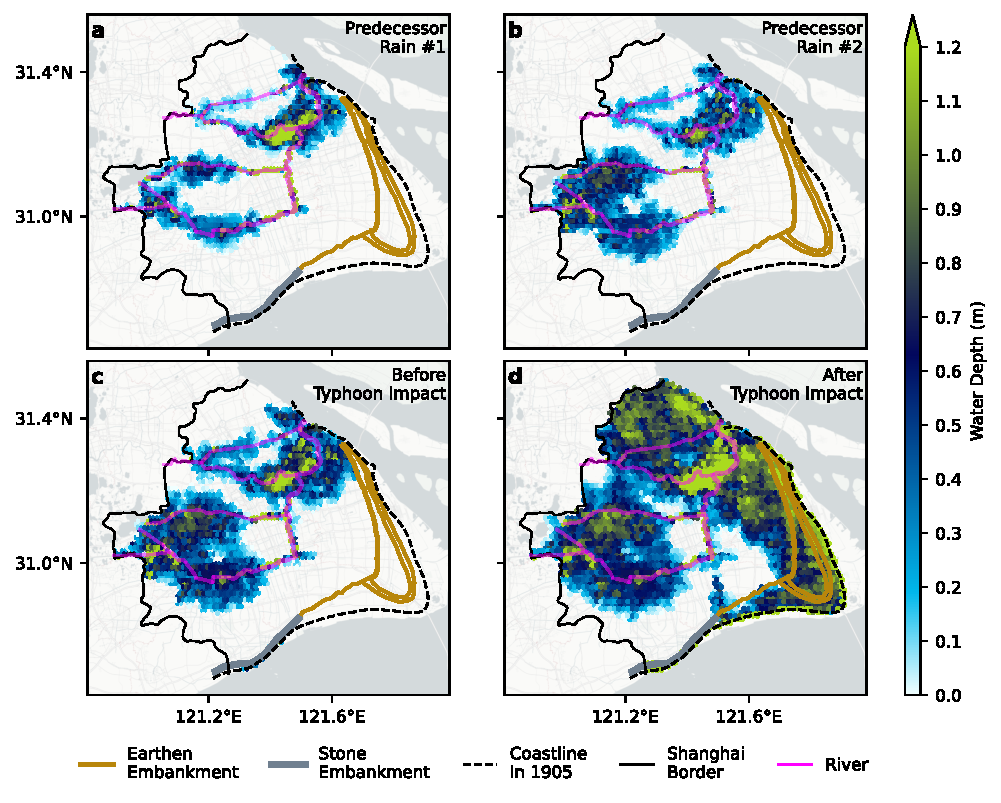
\includegraphics[width=6.5in,height=5.21389in]{media_main/media/image4.pdf}

Figure 2. Simulated water depth (a) after the first predecessor rain
event on August 21\textsuperscript{st}, (b) after the second predecessor
rain event on August 28\textsuperscript{th}, (c) before typhoon impact
on September 1\textsuperscript{st}, and (d) after typhoon impact on
September 2\textsuperscript{nd}. The blue shading shows water depth (m),
with the brown and gray lines highlighting the locations of earthen and
stone embankments in 1905, respectively, and magenta line denoting major
rivers passing Shanghai. The black dashed line shows the coastline in
1905. The thin black solid show the modern Shanghai land border.

Figure 3. Simulated water depth relative to the control experiment by
removing individual hydrological factors. (a) The first predecessor
rainfall event on August 21\textsuperscript{st} removed. (b) The second
predecessor rainfall event on August 28\textsuperscript{th} removed. (c)
Neap high tide a week before replacing spring high tide during the
typhoon impact. (d) Stone embankment replaced by earthen embankment. The
line denotations are the same as in Figure 2.

Table 1. Statistics of flooded area and changes in water depth in all
simulations. The control simulation is forced by two predecessor
rainfall events (\#1 and \#2), spring high tide, and the existence of a
stone embankment. All the other sensitivity experiences are conducted by
removing each forcing. The areal statistics are relative to the whole
Shanghai region. The 95\textsuperscript{th} percentiles are not given if
the change in area showing decreased/increased depth is less than 5\%.

{\def\LTcaptype{none} % do not increment counter
\begin{longtable}[]{@{}
  >{\centering\arraybackslash}p{(\linewidth - 10\tabcolsep) * \real{0.2295}}
  >{\centering\arraybackslash}p{(\linewidth - 10\tabcolsep) * \real{0.1453}}
  >{\centering\arraybackslash}p{(\linewidth - 10\tabcolsep) * \real{0.1555}}
  >{\centering\arraybackslash}p{(\linewidth - 10\tabcolsep) * \real{0.1555}}
  >{\centering\arraybackslash}p{(\linewidth - 10\tabcolsep) * \real{0.1555}}
  >{\centering\arraybackslash}p{(\linewidth - 10\tabcolsep) * \real{0.1586}}@{}}
\toprule\noalign{}
\begin{minipage}[b]{\linewidth}\centering
\end{minipage} & \begin{minipage}[b]{\linewidth}\centering
Control
\end{minipage} & \begin{minipage}[b]{\linewidth}\centering
No rain \#1
\end{minipage} & \begin{minipage}[b]{\linewidth}\centering
No rain \#2
\end{minipage} & \begin{minipage}[b]{\linewidth}\centering
Neap high tide
\end{minipage} & \begin{minipage}[b]{\linewidth}\centering
No stone embankment
\end{minipage} \\
\midrule\noalign{}
\endhead
\bottomrule\noalign{}
\endlastfoot
Flooded area of Shanghai & 73\% & 73\% & 71\% & 50\% & 78\% \\
Area showing \textbf{decreased} \textbf{depth} & --- & 11\% & 63\% &
73\% & 26\% \\
95\textsuperscript{th} percentile \textbf{decrease} (m) & --- & 0.08 &
0.11 & 1.02 & 0.42 \\
Area showing

\textbf{increased} \textbf{depth} & --- & 1\% & 2\% & 2\% & 12\% \\
95\textsuperscript{th} percentile \textbf{increase} (m) & --- & --- &
--- & --- & 0.61 \\
\end{longtable}
}

\textbf{Reference}

1. Neumann, B., Vafeidis, A. T., Zimmermann, J. \& Nicholls, R. J.
Future Coastal Population Growth and Exposure to Sea-Level Rise and
Coastal Flooding - A Global Assessment. \emph{PLOS ONE} \textbf{10},
e0118571 (2015).

2. Hinkel, J. \emph{et al.} Coastal flood damage and adaptation costs
under 21st century sea-level rise. \emph{Proceedings of the National
Academy of Sciences} \textbf{111}, 3292--3297 (2014).

3. McGranahan, G., Balk, D. \& Anderson, B. The rising tide: assessing
the risks of climate change and human settlements in low elevation
coastal zones. \emph{Environment \& Urbanization} \textbf{19}, 17--37
(2007).

4. Cazenave, A. \& Cozannet, G. L. Sea level rise and its coastal
impacts. \emph{Earth's Future} \textbf{2}, 15--34 (2014).

5. Nicholls, R. J. \& Cazenave, A. Sea-Level Rise and Its Impact on
Coastal Zones. \emph{Science} \textbf{328}, 1517--1520 (2010).

6. Batstone, C. \emph{et al.} A UK best-practice approach for extreme
sea-level analysis along complex topographic coastlines. \emph{Ocean
Engineering} \textbf{71}, 28--39 (2013).

7. Toro, G. R., Resio, D. T., Divoky, D., Niedoroda, A. Wm. \& Reed, C.
Efficient joint-probability methods for hurricane surge frequency
analysis. \emph{Ocean Engineering} \textbf{37}, 125--134 (2010).

8. Yang, K., Paramygin, V. \& Sheng, Y. P. An objective and efficient
method for estimating probabilistic coastal inundation hazards.
\emph{Nat Hazards} \textbf{99}, 1105--1130 (2019).

9. Wahl, T., Jain, S., Bender, J., Meyers, S. D. \& Luther, M. E.
Increasing risk of compound flooding from storm surge and rainfall for
major US cities. \emph{Nature Clim Change} \textbf{5}, 1093--1097
(2015).

10. Ward, P. J. \emph{et al.} Dependence between high sea-level and high
river discharge increases flood hazard in global deltas and estuaries.
\emph{Environ. Res. Lett.} \textbf{13}, 084012 (2018).

11. Zscheischler, J. \emph{et al.} Future climate risk from compound
events. \emph{Nature Clim Change} \textbf{8}, 469--477 (2018).

12. Hendry, A. \emph{et al.} Assessing the characteristics and drivers
of compound flooding events around the UK coast. \emph{Hydrology and
Earth System Sciences} \textbf{23}, 3117--3139 (2019).

13. Moftakhari, H., Schubert, J. E., AghaKouchak, A., Matthew, R. A. \&
Sanders, B. F. Linking statistical and hydrodynamic modeling for
compound flood hazard assessment in tidal channels and estuaries.
\emph{Advances in Water Resources} \textbf{128}, 28--38 (2019).

14. Moftakhari, H. R., Salvadori, G., AghaKouchak, A., Sanders, B. F. \&
Matthew, R. A. Compounding effects of sea level rise and fluvial
flooding. \emph{Proceedings of the National Academy of Sciences}
\textbf{114}, 9785--9790 (2017).

15. Nasr, A. A., Wahl, T., Rashid, M. M., Camus, P. \& Haigh, I. D.
Assessing the dependence structure between oceanographic, fluvial, and
pluvial flooding drivers along the United States coastline.
\emph{Hydrology and Earth System Sciences} \textbf{25}, 6203--6222
(2021).

16. Peña, F. \emph{et al.} Compound flood modeling framework for
surface--subsurface water interactions. \emph{Nat. Hazards Earth Syst.
Sci.} \textbf{22}, 775--793 (2022).

17. Gori, A., Lin, N. \& Xi, D. Tropical Cyclone Compound Flood Hazard
Assessment: From Investigating Drivers to Quantifying Extreme Water
Levels. \emph{Earth's Future} \textbf{8}, (2020).

18. Liu, Q., Xu, H. \& Wang, J. Assessing tropical cyclone compound
flood risk using hydrodynamic modelling: a case study in Haikou City,
China. \emph{Nat. Hazards Earth Syst. Sci.} \textbf{22}, 665--675
(2022).

19. Huang, W. \emph{et al.} Compounding factors for extreme flooding
around Galveston Bay during Hurricane Harvey. \emph{Ocean Modelling}
\textbf{158}, 101735 (2021).

20. Valle-Levinson, A., Olabarrieta, M. \& Heilman, L. Compound flooding
in Houston-Galveston Bay during Hurricane Harvey. \emph{Science of The
Total Environment} \textbf{747}, 141272 (2020).

21. Li, X. \emph{et al.} Impacts of urbanization, antecedent rainfall
event, and cyclone tracks on extreme floods at Houston reservoirs during
Hurricane Harvey. \emph{Environ. Res. Lett.} \textbf{15}, 124012 (2020).

22. Vousdoukas, M. I. \emph{et al.} Global probabilistic projections of
extreme sea levels show intensification of coastal flood hazard.
\emph{Nat Commun} \textbf{9}, 2360 (2018).

23. Le Bars, D. Uncertainty in Sea Level Rise Projections Due to the
Dependence Between Contributors. \emph{Earth's Future} \textbf{6},
1275--1291 (2018).

24. Syvitski, J. P. M. \emph{et al.} Sinking deltas due to human
activities. \emph{Nature Geosci} \textbf{2}, 681--686 (2009).

25. Louie, K.-S. \& Liu, K.-B. Earliest Historical Records of Typhoons
in China. \emph{Journal of Historical Geography} \textbf{29}, 299--316
(2003).

26. Yu, F., Chen, Z., Ren, X. \& Yang, G. Analysis of historical floods
on the Yangtze River, China: Characteristics and explanations.
\emph{Geomorphology} \textbf{113}, 210--216 (2009).

27. Li, W., Wen, J., Xu, B., Li, X. \& Du, S. Integrated Assessment of
Economic Losses in Manufacturing Industry in Shanghai Metropolitan Area
Under an Extreme Storm Flood Scenario. \emph{Sustainability}
\textbf{11}, 126 (2019).

28. Du, S. \emph{et al.} Hard or soft flood adaptation? Advantages of a
hybrid strategy for Shanghai. \emph{Global Environmental Change}
\textbf{61}, 102037 (2020).

29. Shan, X. \emph{et al.} Using Multidisciplinary Analysis to Develop
Adaptation Options against Extreme Coastal Floods. \emph{Int J Disaster
Risk Sci} \textbf{13}, 577--591 (2022).

30. Froc, L. \emph{Atlas of the Tracks of 620 Typhoons, 1893-1918}.
(l'Orphelinat de Tòu-sè-w, 1920).

31. Kernkamp, H. W. J., Van Dam, A., Stelling, G. S. \& De Goede, E. D.
Efficient scheme for the shallow water equations on unstructured grids
with application to the Continental Shelf. \emph{Ocean Dynamics}
\textbf{61}, 1175--1188 (2011).

32. Xiqing, C. Sea-Level Changes Since the Early 1920's from the Long
Records of Two Tidal Gauges in Shanghai, China. \emph{Journal of Coastal
Research} \textbf{7}, (1991).

33. Atkinson, G. D. \& Holliday, C. R. Tropical Cyclone Minimum Sea
Level Pressure/Maximum Sustained Wind Relationship for the Western North
Pacific. \emph{Monthly Weather Review} \textbf{105}, 421--427 (1977).

34. Knaff, J. A. \& Zehr, R. M. Reexamination of Tropical Cyclone
Wind--Pressure Relationships. \emph{Weather and Forecasting}
\textbf{22}, 71--88 (2007).

35. Ke, Q., Jonkman, S. N., van Gelder, P. H. A. J. M. \& Bricker, J. D.
Frequency analysis of storm-surge-induced flooding for the Huangpu River
in Shanghai, China. \emph{Journal of Marine Science and Engineering}
\textbf{6}, (2018).

36. Du, S. \emph{et al.} Hard or soft flood adaptation? Advantages of a
hybrid strategy for Shanghai. \emph{Global Environmental Change}
\textbf{61}, 102037 (2020).

37. Kirezci, E. \emph{et al.} Projections of global-scale extreme sea
levels and resulting episodic coastal flooding over the 21st Century.
\emph{Sci Rep} \textbf{10}, 11629 (2020).

38. A new Great Wall. \emph{The Economist} 49--51 (2023).

39. Maduwantha, P. \emph{et al.} Generating Boundary Conditions for
Compound Flood Modeling in a Probabilistic Framework. Preprint at
https://doi.org/10.5194/egusphere-2025-1557 (2025).

40. Gori, A., Lin, N., Xi, D. \& Emanuel, K. Tropical cyclone
climatology change greatly exacerbates US extreme rainfall--surge
hazard. \emph{Nat. Clim. Chang.} \textbf{12}, 171--178 (2022).

41. Smith, A. B. \& Matthews, J. L. Quantifying uncertainty and variable
sensitivity within the US billion-dollar weather and climate disaster
cost estimates. \emph{Nat Hazards} \textbf{77}, 1829--1851 (2015).

42. Emanuel, K. Increasing Destructiveness of Tropical Cyclones over the
Past 30 Years. \emph{Nature} \textbf{436}, 686--688 (2005).

43. Gori, A., Lin, N., Xi, D. \& Emanuel, K. Tropical cyclone
climatology change greatly exacerbates US extreme rainfall--surge
hazard. \emph{Nature Climate Change} \textbf{12}, 171--178 (2022).

44. Wang, S., Toumi, R., Czaja, A. \& Kan, A. V. An analytic model of
tropical cyclone wind profiles. \emph{Quarterly Journal of the Royal
Meteorological Society} \textbf{141}, 3018--3029 (2015).

45. Wang, S. \& Toumi, R. On the relationship between hurricane cost and
the integrated wind profile. \emph{Environmental Research Letters}
\textbf{11}, 114005 (2016).

46. Holland, G. J. An Analytic Model of the Wind and Pressure Profiles
in Hurricanes. \emph{Monthly Weather Review} \textbf{108}, 1212--1218
(1980).

47. Holland, G. J., Belanger, J. I. \& Fritz, A. A Revised Model for
Radial Profiles of Hurricane Winds. \emph{Monthly Weather Review}
\textbf{138}, 4393--4401 (2010).

\end{document}
